% Write about what kind of queries you are expect to get in this system

\section{Database execution }
% What are the execution methods when these functionalities are carried out
In this section, we go through the execution methods of the database based on the transactions that have been carried out within the system. This also shows where the data is expected to roughly end up, however this will be explained in greater detail along with the diagrams which will be found later in this document.

Stakeholders and users have to be aware that due to lightweight database files are stored locally in each users' computer, there are a number of databases involve when the transactions are carried out. The reason why it is designed this way is to ensure and avoid any malicious activities conducted especially by the server. 

\subsection{User adds post, comment and event}
When a user adds a content into Turtlenet such as posts, comments and events, the system is expected to capture these details and add them into its respective tables. The database system is expected to log the posts, comments and events by capturing the time and date when the transaction is carried out.

\subsection{User creates and sends message to another user}
As when the user creates a message then sends it, the database system is expected to store the message and log it by recording its date and time of which the message is sent. Other details like the reciever's user\_id are inserted into the database well.

\subsection{User sends a friend request to another user}
When the user sends a request to others, this request will be sent and the details will be captured and recorded into the other user's local database file under the friend request table. This will be stored in this table until which the user decides to either accept or reject the invitation.

\subsection{User receives a friend request from another user}
Another situation with the friend request is when a user receives a friend request, this time the information such as the public key will be recorded into the user's local database until which the user decides to do something either accept or reject it.

\subsection{A user adds a relation}
When a user adds a relation, the details of this related user will be captured, such as his profile, and will be added into the users table. From then on, the user can see his relation's profile information. 

\subsection{User receives a message} 
As the user receives a message, it will be stored in the message table along with other details such as the date and time, and the sender's details.

\subsection{User receives a friend request}
The user will be notified when a friend request is sent. The details of the person who sends the request will be recorded in the database. The user has two options to deal with a friend request, either to accept or reject it. Once it is accepted, the profile details of the sender will be stored in the user's local database, same goes to the user's details store on the sender's local database.

\clearpage

\section{Table layout of the database}
% Aishah says: I will redo this pile (of shit designed database) once I clarify with other team members on the functionalities of Tu-tu-roo-net.
NB: Public keys are 217 characters long, all id's are auto-incremented.

\begin{table}[!ht]
\caption{you}
\centering
\begin{tabular}{c c c}
\hline\hline
Name               & Datatype    & Key \\
\hline
username           & VARCHAR(25) & PK   \\
name               & VARCHAR(30) &      \\
birthday           & DATE        &      \\
sex                & VARCHAR(1)  &      \\
email              & VARCHAR(30) &      \\
public\_key        & VARCHAR(8)  &      \\
\hline
\end{tabular}
\label{table:nonlin}
\end{table}

\begin{table}[!ht]
\caption{user}
\centering
\begin{tabular}{c c c}
\hline\hline
Name               & Datatype    & Key \\
\hline
user\_id           & VARCHAR(8)  & PK \\  % 64-bit has key public key
username           & VARCHAR(25) &    \\
name               & VARCHAR(30) &    \\
birthday           & DATE        &    \\
sex                & VARCHAR(1)  &    \\
email              & VARCHAR(30) &    \\
\hline
\end{tabular}
\label{table:nonlin}
\end{table}

\begin{table}[!ht]
\caption{is\_in\_category}
\centering
\begin{tabular}{c c c}
\hline\hline
Name               & Datatype    & Key \\
\hline
is\_in\_id         & INT(10)     & PK   \\
category\_id       & INT(10)     & FK   \\
user\_id           & INT(5)      & FK   \\
\hline
\end{tabular}
\label{table:nonlin}
\end{table}

\begin{table}[!ht]
\caption{category}
\centering
\begin{tabular}{c c c}
\hline\hline
Name               & Datatype    & Key \\
\hline
category\_id       & INT(10)     & PK  \\
name               & VARCHAR(30) &     \\
\hline
\end{tabular}
\label{table:nonlin}
\end{table}



\begin{table}[!ht]
\caption{private\_message}
\centering
\begin{tabular}{c c c}
\hline\hline
Name               & Datatype    & Key \\
\hline
message\_id        & INT(10)     & PK  \\
from               & VARCHAR(8)  &     \\
to                 & VARCHAR(8)  &     \\
content            & VARCHAR(50) &     \\
time               & DATE        &     \\
\hline
\end{tabular}
\label{table:nonlin}
\end{table}

\begin{table}[!ht]
\caption{wall\_post}
\centering
\begin{tabular}{c c c}
\hline\hline
Name                    & Datatype    & Key \\
\hline
wall\_id                & INT(10)     & PK  \\
from                    & VARCHAR(8)  & FK  \\
to                      & VARCHAR(8)  & FK  \\
permission\_to          & VARCHAR(8)  & FK  \\
content                 & VARCHAR(50) &     \\
time                    & DATE        &     \\
\hline
\end{tabular}
\label{table:nonlin}
\end{table}

\begin{table}[!ht]
\caption{has\_comment}
\centering
\begin{tabular}{c c c}
\hline\hline
Name               & Datatype    & Key \\
\hline
comment\_id        & INT(10)     & PK  \\
post\_id           & INT(10)     & FK  \\
user\_id           & VARCHAR(8)  & FK  \\
comment\_time      & DATE        &     \\
\hline
\end{tabular}
\label{table:nonlin}
\end{table}

\begin{table}[!ht]
\caption{has\_like}
\centering
\begin{tabular}{c c c}
\hline\hline
Name               & Datatype    & Key \\
\hline
like\_id           & INT(10)     & PK  \\
post\_id           & INT(8)      & FK  \\
user\_id           & VARCHAR(8)  & FK  \\
\hline
\end{tabular}
\label{table:nonlin}
\end{table}

\begin{table}[!ht]
\caption{events}
\centering
\begin{tabular}{c c c}
\hline\hline
Name                    & Datatype    & Key \\
\hline
event\_id               & INT(10)     & PK  \\
title                   & VARCHAR(10) &     \\
content                 & VARCHAR(40) &     \\
from                    & VARCHAR(8)  & FK  \\
permission\_allowed\_to & VARCHAR(8)  & FK  \\
\hline
\end{tabular}
\label{table:nonlin}
\end{table}

\begin{table}[!ht]
\caption{friend\_request}
\centering
\begin{tabular}{c c c}
\hline\hline
Name               & Datatype    & Key \\
\hline
public\_key        & VARCHAR(8)  & PK  \\
request\_time      & DATE        &     \\
request\_react     & VARCHAR(10) &     \\ % pending, accepted, rejected
\hline
\end{tabular}
\label{table:nonlin}
\end{table}

\begin{table}[!ht]
\caption{login\_logout\_log}
\centering
\begin{tabular}{c c c}
\hline\hline
Name               & Datatype    & Key \\
\hline
log\_id            & INT(10)     & PK  \\
login\_time        & DATE        &     \\
logout\_time       & DATE        &     \\
\hline
\end{tabular}
\label{table:nonlin}
\end{table}

\clearpage

\begin{landscape}
\begin{figure}[h]
    
    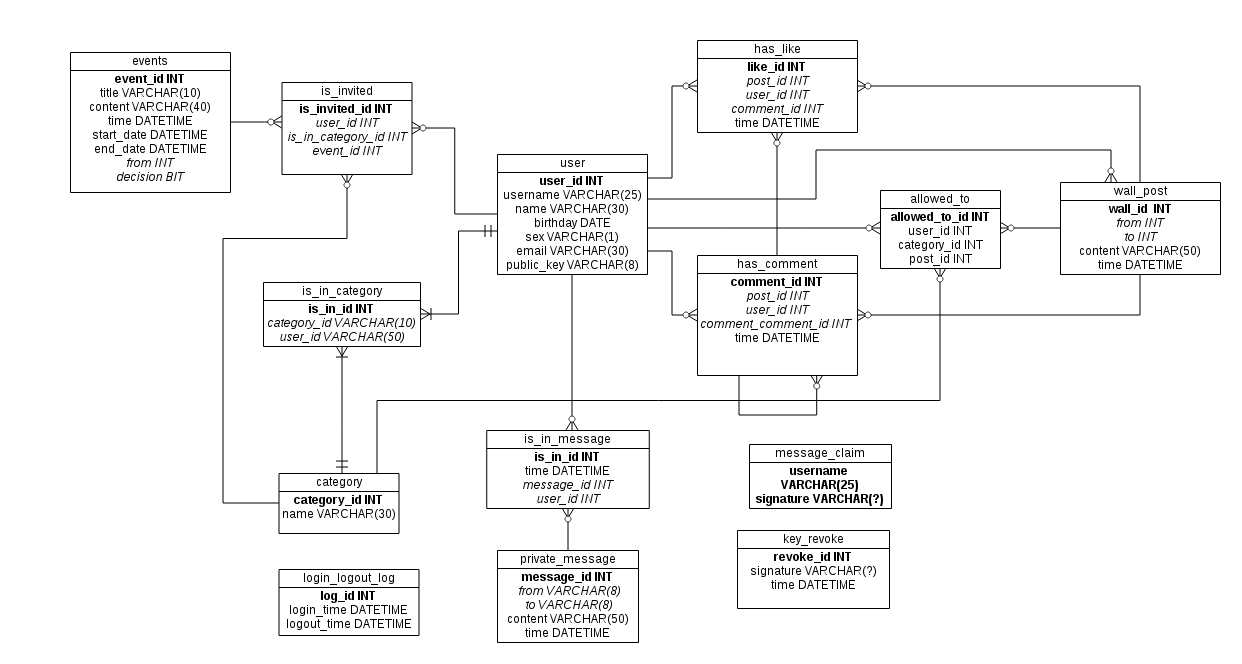
\includegraphics[height=0.7\textwidth]{images/design/project_er_diagram.png}
    \caption{Database Entity Relationship diagram}
    \label{fig:db_er_diag}
\end{figure}
\end{landscape}